\subsection{\RU{Запись за пределы массива}\EN{Writing behind array bounds}}

\RU{Итак, мы прочитали какое-то число из стека явно \IT{нелегально}, а что если мы запишем?}
\EN{OK, we read some values from the stack \IT{illegally} but what if we could write something to it?}

\RU{Вот что мы пишем:}\EN{Here is what we will write:}

\lstinputlisting{patterns/13_arrays/2_BO/w.c}

\subsubsection{MSVC}

\RU{И вот что имеем на ассемблере:}\EN{And what we've got:}

\lstinputlisting[caption=\NonOptimizing MSVC 2008]{patterns/13_arrays/2_BO/w.asm.\LANG}

\RU{Запускаете скомпилированную программу, и она падает. Немудрено. Но давайте теперь узнаем, где именно.}
\EN{Run compiled program and its crashing. No wonder. Let's see, where exactly it is crashing.}

\clearpage
\index{\olly}

\RU{Загружаем в}\EN{Let's load into} \olly, \RU{трассируем, пока запишутся все 30 элементов}
\EN{trace until all 30 elements are written}:

\begin{figure}[H]
\centering
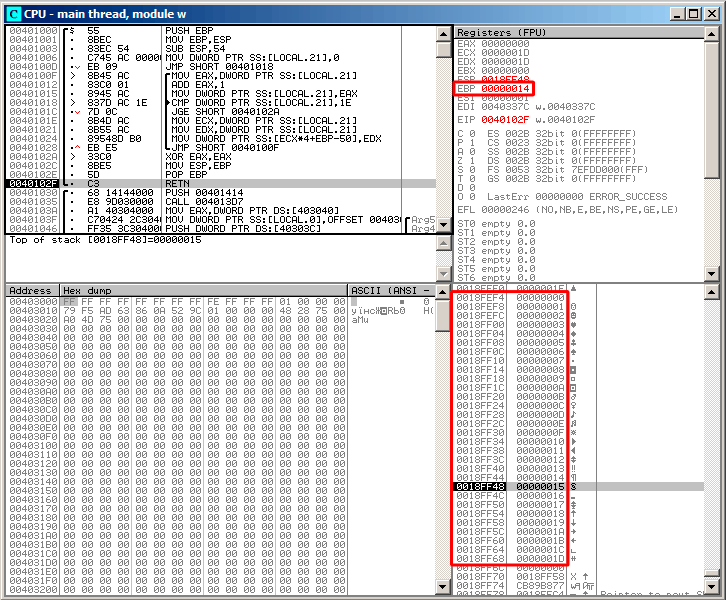
\includegraphics[scale=\FigScale]{patterns/13_arrays/2_BO/olly_w1.png}
\caption{\olly: \RU{после восстановления EBP}\EN{after restoring value of EBP}}
\label{fig:array_BO_olly_w1}
\end{figure}

\clearpage
\RU{Доходим до конца ф-ции}\EN{Trace until the function end}:

\begin{figure}[H]
\centering
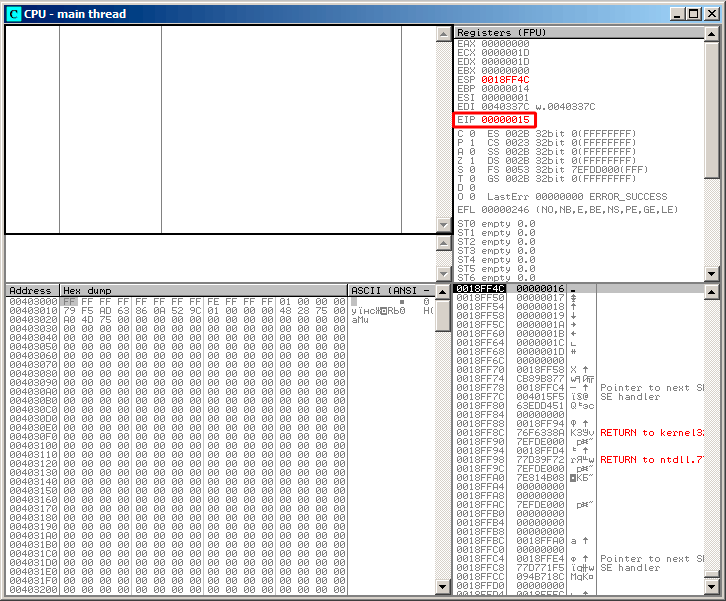
\includegraphics[scale=\FigScale]{patterns/13_arrays/2_BO/olly_w2.png}
\caption{\olly: \RU{EIP восстановлен, но \olly не может дизассемблировать по адресу 0x15}
\EN{EIP is restored, but \olly can't disassemble at 0x15}}
\label{fig:array_BO_olly_w2}
\end{figure}

\RU{Итак, следите внимательно за регистрами.}
\EN{Now please keep your eyes on registers.}

\RU{\EIP теперь 0x15. Это явно нелегальный адрес для кода ~--- по крайней мере, win32-кода! 
Мы там как-то очутились, причем, сами того не хотели. Интересен также тот факт, что в \EBP хранится 0x14, 
а в \ECX и \EDX ~--- 0x1D.}
\EN{\EIP is 0x15 now. It is not legal address for code~---at least for win32 code!
We trapped there somehow against our will.
It is also interesting fact the \EBP register contain 0x14,
\ECX and \EDX{}~---0x1D.}

\RU{И еще немного изучим разметку стека.}\EN{Let's study stack layout more.}

\RU{После того как управление передалось в \main, в стек было сохранено значение \EBP. 
Затем, для массива + переменной $i$ было выделено $84$ байта. Это \TT{(20+1)*sizeof(int)}. 
\ESP сейчас указывает на переменную \TT{\_i} в локальном стеке и при исполнении следующего \TT{PUSH что-либо}, 
\IT{что-либо} появится рядом с \TT{\_i}.}
\EN{After control flow was passed into \TT{\main}, the value in the \EBP register was saved on the stack.
Then, $84$ bytes was allocated for array and $i$ variable.
That's \TT{(20+1)*sizeof(int)}.
The \ESP pointing now to the \TT{\_i} variable in the local stack and after execution of next \TT{PUSH something},
\IT{something} will be appeared next to \TT{\_i}.}

\RU{Вот так выглядит разметка стека пока управление находится внутри}
\EN{That's stack layout while control is inside} \main:

\begin{center}
\begin{tabular}{ | l | l | }
\hline
  \TT{ESP}    & \RU{4 байта выделенных для переменной $i$}\EN{4 bytes allocated for $i$ variable} \\
\hline
  \TT{ESP+4}  & \RU{80 байт выделенных для массива \TT{a[20]}}\EN{80 bytes allocated for \TT{a[20]} array} \\
\hline
  \TT{ESP+84} & \RU{сохраненное значение \EBP}\EN{saved \EBP value} \\
\hline
  \TT{ESP+88} & \RU{адрес возврата}\EN{returning address} \\
\hline
\end{tabular}
\end{center}

\RU{Выражение \TT{a[19]=чего\_нибудь} записывает последний \Tint в пределах массива (пока что в пределах!)}
\EN{\TT{a[19]=something} statement writes last \Tint in array bounds (in bounds so far!)}

\RU{Выражение \TT{a[20]=чего\_нибудь} записывает \IT{чего\_нибудь} на место где сохранено значение \EBP.}
\EN{\TT{a[20]=something} statement writes \IT{something} to the place where value of the \EBP is saved.}

\RU{Обратите внимание на состояние регистров на момент падения процесса. В нашем случае, 
в 20-й элемент записалось значение 20. 
И вот все дело в том, что заканчиваясь, эпилог функции восстанавливал значение \EBP. 
(20 в десятичной системе это как раз 0x14 в шестнадцатеричной). 
Далее выполнилась инструкция \RET, которая на самом деле эквивалентна \TT{POP EIP}.}
\EN{Please take a look at registers state at the crash moment. In our case,
number 20 was written to 20th element. 
By the function ending, function epilogue restores original \EBP value.
(20 in decimal base is 0x14 in hexadecimal).
Then, \RET instruction was executed, which is effectively equivalent to \TT{POP EIP} instruction.}

\RU{Инструкция \RET вытащила из стека адрес возврата (это адрес где-то внутри \ac{CRT}), 
которая вызвала \main), 
а там было записано 21 в десятичной системе, то есть 0x15 в шестнадцатеричной. 
И вот процессор оказался по адресу 0x15, но исполняемого кода там нет, так что случилось исключение.}
\EN{\RET instruction taking returning address from the stack (that is the address inside of \ac{CRT}),
which was called \main),
and 21 was stored there (0x15 in hexadecimal).
The CPU trapped at the address 0x15,
but there is no executable code, so exception was raised.}

\index{\RU{Переполнение буфера}\EN{Buffer overflow}}
\RU{Добро пожаловать! Это называется}
\EN{Welcome! It is called} \IT{buffer overflow}\footnote{\href{http://go.yurichev.com/17132}{wikipedia}}.

\RU{Замените массив \Tint на строку (массив \Tchar), нарочно создайте слишком длинную строку, 
просуньте её в ту программу, 
в ту функцию, которая не проверяя длину строки скопирует её в слишком короткий буфер, 
и вы сможете указать программе, по какому именно адресу перейти. 
Не все так просто в реальности, конечно, но началось все с этого
\footnote{Классическая статья об этом: \cite{Phrack4914}}.}
\EN{Replace \Tint array by string (\Tchar array), create a long string deliberately,
and pass it to the program, to the function which is not checking string length and copies it to short buffer,
and you'll able to point to a program an address to which it must jump.
Not that simple in reality, but that is how it was emerged
\footnote{Classic article about it: \cite{Phrack4914}.}}

\subsubsection{GCC}

\RU{Попробуем то же самое в GCC 4.4.1. У нас выходит такое:}
\EN{Let's try the same code in GCC 4.4.1. We got:}

\lstinputlisting{patterns/13_arrays/2_BO/w_gcc.asm}

\RU{Запуск этого в Linux выдаст:}\EN{Running this in Linux will produce:} \TT{Segmentation fault}.

\index{GDB}
\RU{Если запустить полученное в отладчике GDB, получим:}
\EN{If we run this in GDB debugger, we getting this:}

\begin{lstlisting}
(gdb) r
Starting program: /home/dennis/RE/1 

Program received signal SIGSEGV, Segmentation fault.
0x00000016 in ?? ()
(gdb) info registers
eax            0x0	0
ecx            0xd2f96388	-755407992
edx            0x1d	29
ebx            0x26eff4	2551796
esp            0xbffff4b0	0xbffff4b0
ebp            0x15	0x15
esi            0x0	0
edi            0x0	0
eip            0x16	0x16
eflags         0x10202	[ IF RF ]
cs             0x73	115
ss             0x7b	123
ds             0x7b	123
es             0x7b	123
fs             0x0	0
gs             0x33	51
(gdb) 
\end{lstlisting}

\RU{Значения регистров немного другие чем в примере win32, это потому что разметка стека чуть другая.}
\EN{Register values are slightly different then in win32 example
since stack layout is slightly different too.}
